\documentclass[11pt,letter]{article}
\usepackage[top=1.00in, bottom=1.0in, left=1.1in, right=1.1in]{geometry}
\renewcommand{\baselinestretch}{1}
\usepackage{graphicx}
\usepackage{natbib}
\usepackage{amsmath}
\usepackage{hyperref}
\usepackage{gensymb}

\def\labelitemi{--}
\parindent=0pt
\parskip=5pt

\begin{document}
\bibliographystyle{/Users/Lizzie/Documents/EndnoteRelated/Bibtex/styles/besjournals}
\renewcommand{\refname}{\CHead{}}

\title{Comparing \emph{Quercus} model from \\ Duputie vs. van der Meersch}
\author{Lizzie, Isabelle Chuine, Ben Cook, Victor van der Meersch}
\date{\today}
\maketitle


\section*{Overview}
For the mean results for \emph{Quercus} we wondered whether the Leaf model parameterization was driving the results. To check this we created an updated file\\
 (\verb|Quercus_robur_ADuputie_updated23June2023.species|) using the leaf model parameterization from Van der Meersch \& Chuine 2023 \\(\verb|cmaes_fit_subset2_rep2.species|). After reviewing the results, Victor replied:

\begin{quote}
I am surprised by the fitness with the updated parameters, which seems veeery low, though there are Quercus indivuals in these latitude.
Maybe it is because we only extracted the leaf/flower parameters from the inverse calibration set?
If it is not time consuming, you could try to run simulations directly with the \verb|cmaes_fit_subset2_rep2.species| file, even though extra precautions must be taken when analysing the results.
\end{quote}

And Isabelle agreed so then I ran with the new parameter set. So in July 2023, I ran with the FULL updated parameters and Duputie. Fitness was higher for the historical data and declined with higher levels of warming (compared to the historical where it was lowest for the lower warming scenarios). 

And then on 15 november 2023, I updated to \verb|Quercus_robur_ADuputie_updated23June2023| which is (similar to our Pinsyl and Fagsyl models) based on `expert opinion,' not on inverse calibration as \verb|cmaes_fit_subset2_rep2.species| is. Below is a comparison of the results between this new `expert opinion' (I refer to this below as an updated model, `updated23June2023') version and the original Duputie that we started with. With this new parameter set, fitness is always very high. 

\section*{Based on historical climate}

See bottom panels of Fig. \ref{fig:histdup}-\ref{fig:histdnew}, fitness is now high across all latitudes with only small effect of MaturationIndex starting around 46\degree N.

For \verb|cmaes_fit_subset2_rep2.species|: trends are similar (MaturationIndex dominates fitness) but now fitness is now low as of latitudes 41 and 44 and higher. I was also struck by how the FruitMatDate changed which now clearly gets later at higher latitudes, and matters to fitness (whereas before neither of these things happened). % see allspp_xypoints_wprint_fruitmatdate_vsfitness.pdf

\begin{figure}[h!]
 \begin{center}
\noindent 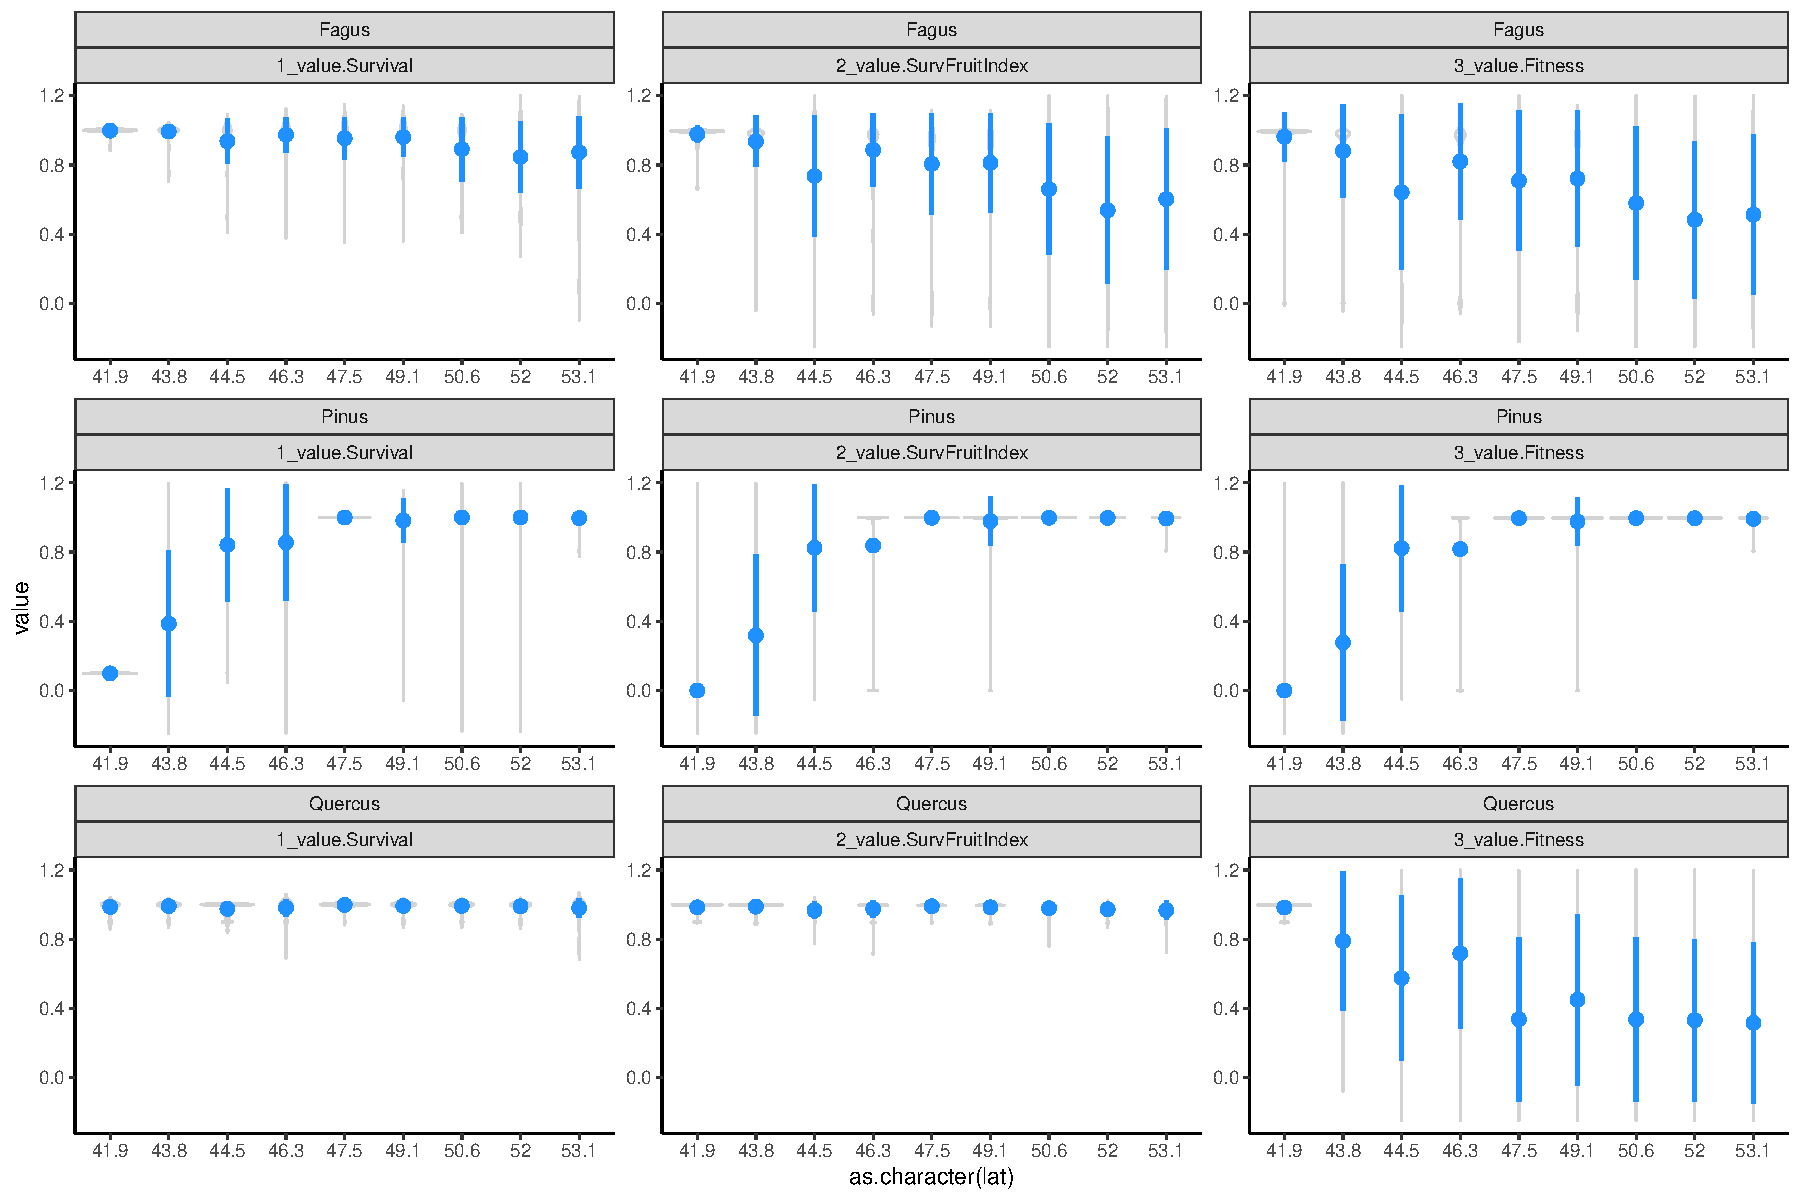
\includegraphics[width=1\textwidth]{..//analyses/graphs/phenofit/historical/fitnessBuildup_DuputieQuercus.pdf}
  \caption{\emph{Quercus} fitness across latitude (historical climate data) based on Duputie parameters. You can see PHENOFIT4 output at \url{https://github.com/lizzieinvancouver/climatehazards/tree/main/analyses/input/phenofit/querob_19512020_Duputie}.}
  \label{fig:histdup}
  \end{center}
\end{figure}

\begin{figure}[h!]
 \begin{center}
\noindent 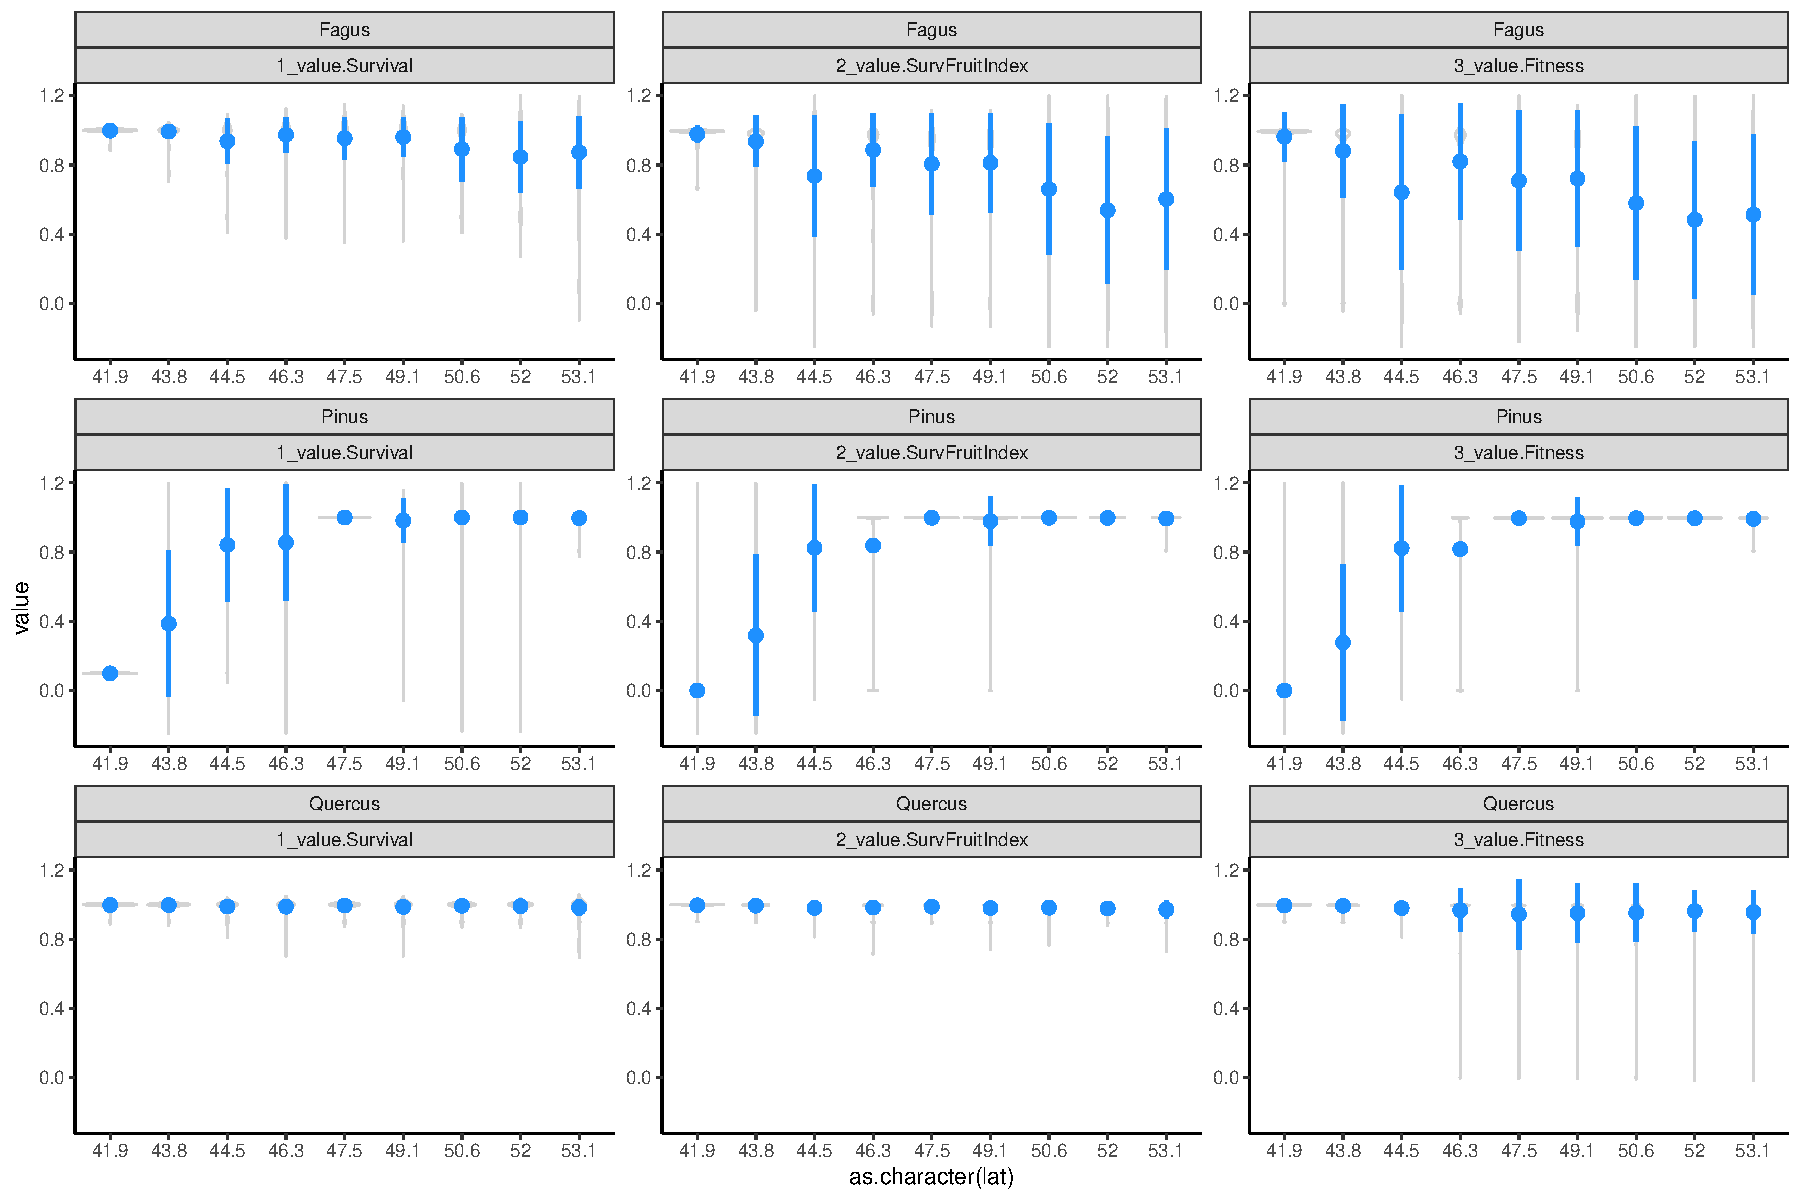
\includegraphics[width=1\textwidth]{..//analyses/graphs/phenofit/historical/fitnessBuildup.pdf}
  \caption{\emph{Quercus} fitness across latitude (historical climate data) based on updated model (ending in `updated23June2023'). You can see PHENOFIT4 output at \url{https://github.com/lizzieinvancouver/climatehazards/tree/main/analyses/input/phenofit/querob_19512020}.}
  \label{fig:histdnew}
  \end{center}
\end{figure}


\section*{Understanding the results using updated model}

On 16 November 2023, Isabelle, Victor and I spent several hours trying to understand why the updated model (ending in `updated23June2023') had such high fitness. I put related files from today in \verb|querob_Nov2023| folder inside analyses/input/phenofit. 

\begin{enumerate}
\item We know the distribution from this parameter set makes sense (see distribution figure in folder) so why is there no decrease in fitness?
\item We used the trace function to follow it carefully and found that with warming you get very early leafout and NEED to UPDATE HERE. 
\item We may see reduced fitness if we lowered WHC.... I am still thinking on this (to 50 or 100; Peuchabon is 50). 
\item The reason the \verb|cmaes_fit_subset2_rep2.species| parameter set makes sense is that it doesn't really! It leads to really weird fruitmatdate because its leafout model has a very low max (compared to the updated model, ending in `updated23June2023'). 
\end{enumerate}

\clearall
\section*{Based on simulated climate with mean warming}

See Fig. \ref{fig:simsmeanDup}-\ref{fig:simsmeanUp}. Fitness is again affected mostly by MaturationIndex, and low at high warming.

\begin{figure}[h!]
 \begin{center}
\noindent 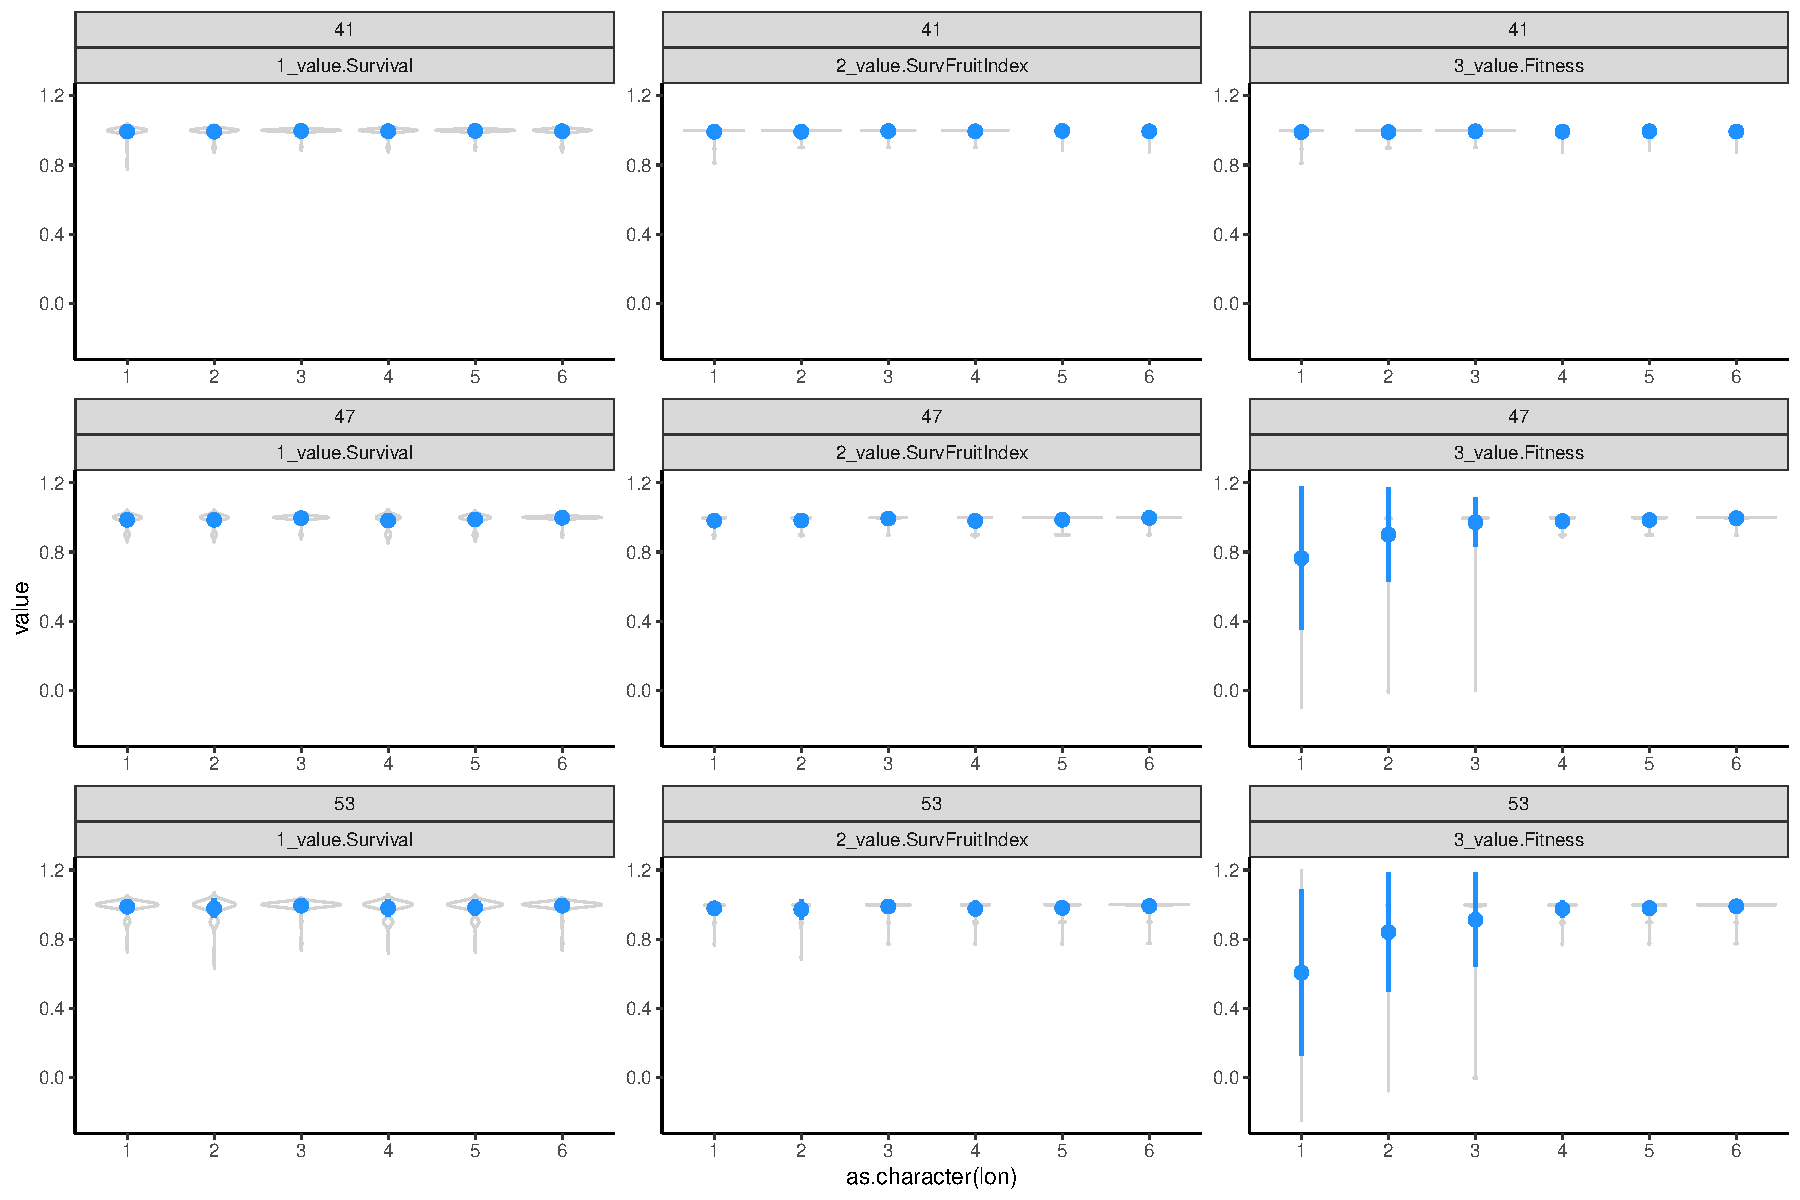
\includegraphics[width=1\textwidth]{..//analyses/graphs/phenofit/sims/querob_Duputie/meansim_3metricsQR.pdf}
  \caption{\emph{Quercus} across 0 (1) to $+$5 (6) mean warming, based on Duputie parameters. To see the underlying components of the model, look for `meansim' QR files at \url{https://github.com/lizzieinvancouver/climatehazards/tree/main/analyses/graphs/phenofit/sims/querob_Duputie}.}
  \label{fig:simsmeanDup}
  \end{center}
\end{figure}

\begin{figure}[h!]
 \begin{center}
\noindent 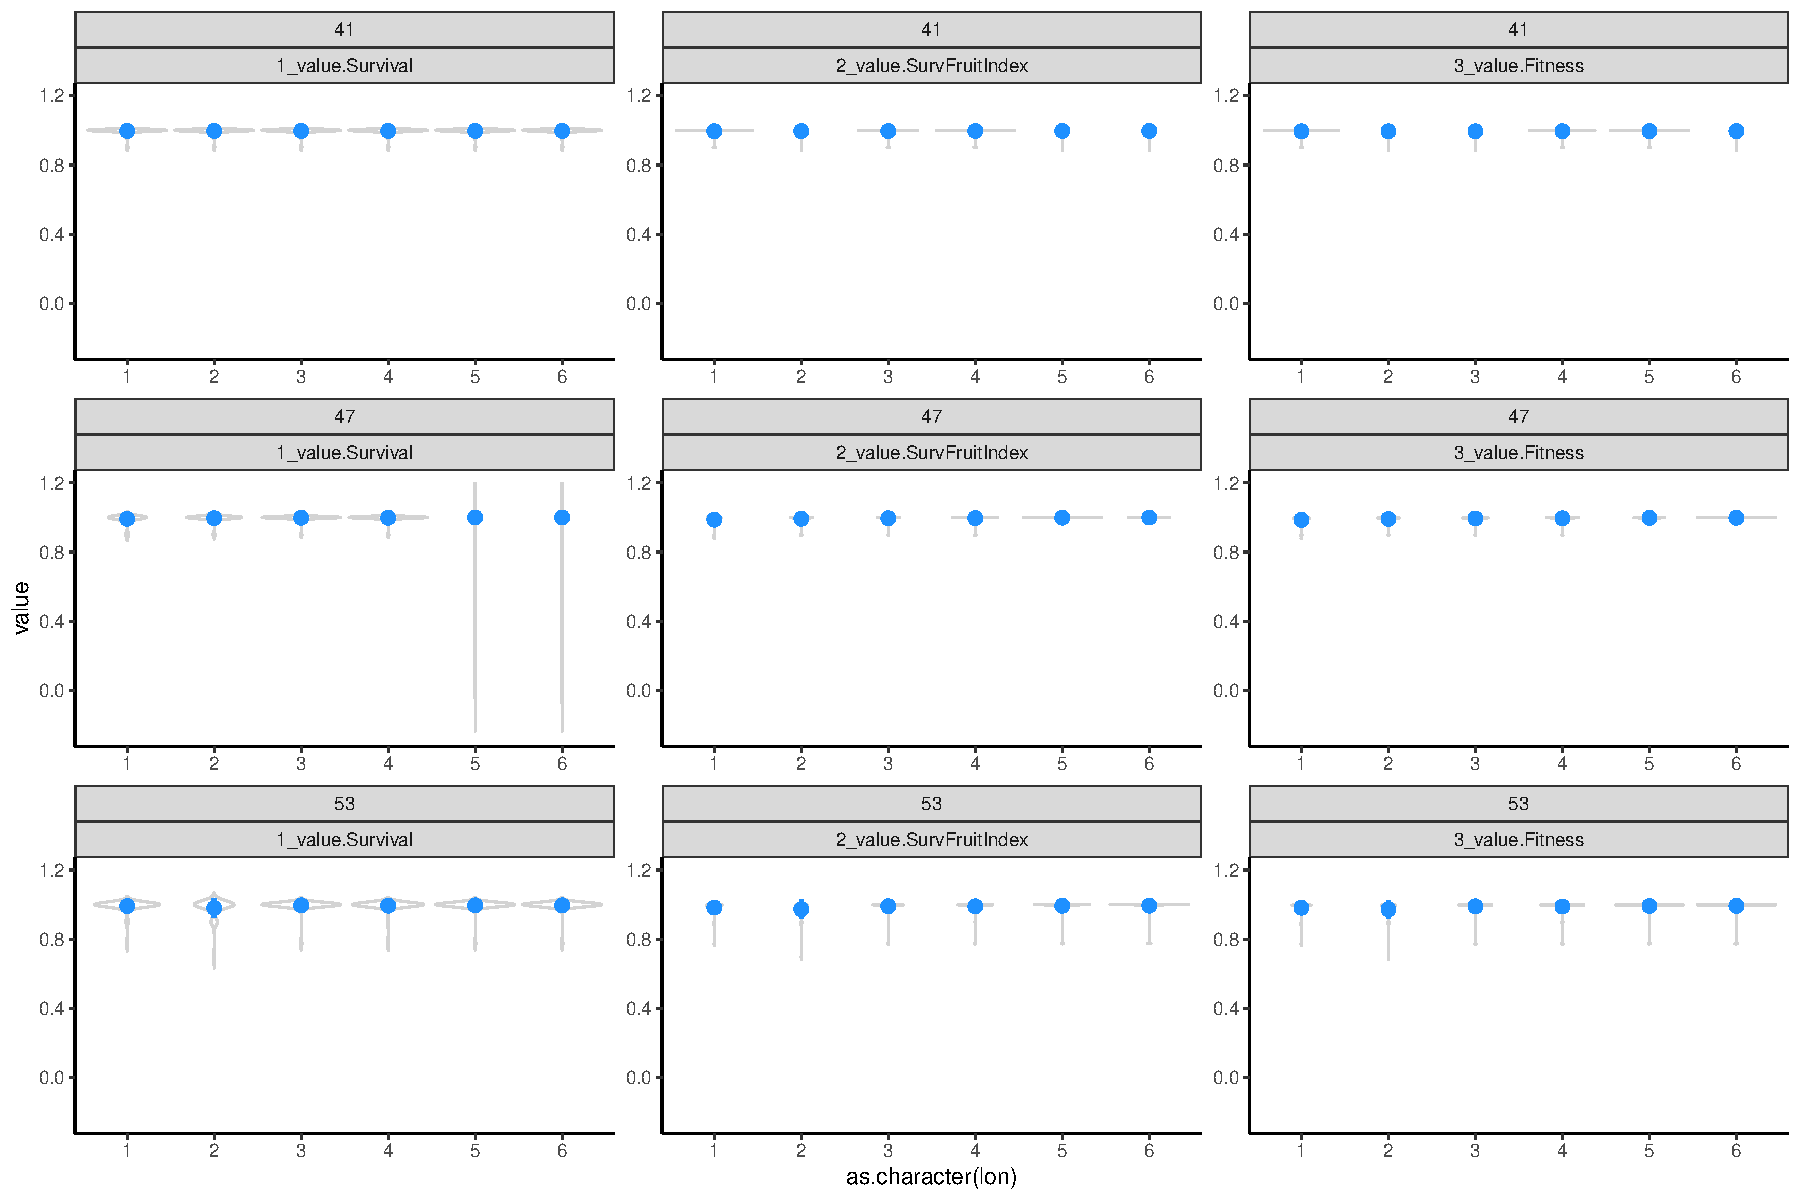
\includegraphics[width=1\textwidth]{..//analyses/graphs/phenofit/sims/metrics3/meansim_3metricsQR.pdf}
  \caption{\emph{Quercus} across 0 (1) to $+$5 (6) mean warming, based on updated model (`updated23June2023'). To see the underlying components of the model, look for `meansim' QR files in \url{https://github.com/lizzieinvancouver/climatehazards/tree/main/analyses/graphs/phenofit/sims}}
  \label{fig:simsmeanUp}
  \end{center}
\end{figure}


\clearall
\section*{Based on simulated climate with changing variance}

See Fig. \ref{fig:simssdDup}-\ref{fig:simssdUp}. Now, fitness is always high, everywhere. 

For \verb|cmaes_fit_subset2_rep2.species|: Fitness dominated by FruitIndex (I think) and decreasing with increasing variance.

\begin{figure}[h!]
 \begin{center}
\noindent \includegraphics[width=1\textwidth]{..//analyses/graphs/phenofit/sims/querob_Duputie/sdsim_3metricsQR.pdf}
  \caption{\emph{Quercus} across changing variance, based on Duputie parameters. To see the underlying components of the model, look for `dssim' QR files at \url{https://github.com/lizzieinvancouver/climatehazards/tree/main/analyses/graphs/phenofit/sims/querob_Duputie}.}
  \label{fig:simssdDup}
  \end{center}
\end{figure}

\begin{figure}[h!]
 \begin{center}
\noindent \includegraphics[width=1\textwidth]{..//analyses/graphs/phenofit/sims/metrics3/sdsim_3metricsQR.pdf}
  \caption{\emph{Quercus} across changing variance, based on updated model (`updated23June2023'). To see the underlying components of the model, look for `sdsim' QR files in \url{https://github.com/lizzieinvancouver/climatehazards/tree/main/analyses/graphs/phenofit/sims}}
  \label{fig:simssdUp}
  \end{center}
\end{figure}



\end{document}
